%%=============================================================================
%% Appendix
%%=============================================================================

\chapter{Using Qiskit yourself}
\label{ch:appendix}

For the practical execution, we preferred to use Anaconda 1.9.12 for all our experiments. By using an environment that was just created for using Qiskit, we could debug way easier as there only were a handful of addition needed.

You will need to pip install, Qiskit, matplotlib, jupyter and Pyscience to have an all-round work environment for creating your own circuits.

Qiskit.org will give a full explanation, if the basics would not suffice.


\section{Setting up your Python-Qiskit environment}

Make sure you are able to execute the commands as shown in figure A.1 to ensure that you are capable to create your own circuits.

\begin{figure}
	\centering
	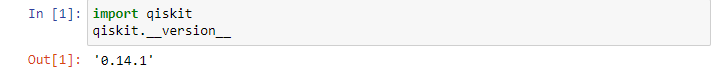
\includegraphics[scale = 0.75]{../Demonstration/img/Qiskit_version.PNG}
	\caption{If you are able to execute this command in your Python environment, you have installed Qiskit successfully.}
\end{figure}

\section{Connecting your Python environment with IBMQ}

If you would like to use the actual devices to perform your tests, you need to create an account on \href{https://quantum-computing.ibm.com/}. Then you need to find your private key and connect it to the environment in a Jupyter notebook as seen in figure A.2. This key will be used each time you send off a circuit to the IBMQ quantum devices, the use of these devices is \textit{free of charge}.

\begin{figure}
	\centering
	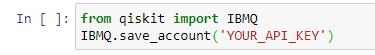
\includegraphics[scale = 0.75]{../Demonstration/img/IBMQ.PNG}
	\caption{The necessary code to connect your Python environment to the external quantum devices.}
\end{figure}


\section{Running the quantum decoherence example}
This section will show the simple way that you can show quantum decoherence taken an effect on your circuits. We will put 1 qubit in an elevated $\ket{1}$ state followed up with a measurement and then send it off to a quantum device.

This are the needed imports for the basic example.

\begin{verbatim}[frame=single]
from qiskit import(
QuantumCircuit,
execute, 
IBMQ,
Aer)
import numpy as np
from qiskit.visualization import plot_histogram
\end{verbatim}

Here we create a quantum register of 1 qubit and apply a Pauli-X gate, followed up by a measurement to a classical register.

\begin{verbatim}[frame=single]
circuit = QuantumCircuit(1,1)
circuit.x(0)
circuit.measure(0,0)
\end{verbatim}

Using matplotlib will result in a much cleaner output of the circuit.

\begin{verbatim}[frame=single]
circuit.draw(output= "mpl")
\end{verbatim}

These are the needed actions to actually set up your device. You will need to choose your ibmq-device on the website where you have signed up for an IBMQ-account.

\begin{verbatim}[frame=single]
IBMQ.load_account()
prov = IBMQ.get_provider(hub='ibm-q')
device = prov.get_backend('ibmq_armonk')
\end{verbatim}

Here we actually send off the circuit towards our device.

\begin{verbatim}[frame=single]
job = execute(circuit, backend = device, shots = 1024)
from qiskit.tools.monitor import job_monitor
job_monitor(job)
result = job.result()
plot_histogram(result.get_counts())
\end{verbatim}

\section{Running the practical 3-SAT example}

In this part, we will showcase the code of the practical portion of this paper where we solved a 3-SAT problem using Qiskit.

First we will perform the algorithm through the use of the simulator, then we will send the circuit off to an IBM device capable of handling the large circuit. (13 qubits needed at the least)

\begin{verbatim}[frame=single]
import numpy as np
import matplotlib as plt
from qiskit import *
from qiskit import BasicAer
from qiskit.visualization import plot_histogram
%config InlineBackend.figure_format = 'svg'
from qiskit.aqua import QuantumInstance
from qiskit.aqua.algorithms import Grover
from qiskit.aqua.components.oracles import LogicalExpressionOracle, TruthTableOracle
\end{verbatim}

This is the specific encoding that is used for encoding a Boolean satisfiability problem into the Grover search algorithm.

\begin{verbatim}[frame=single]
input_3sat = '''
c example DIMACS-CNF 3-SAT
p cnf 3 5
-1 2 -3 0
1 -2 -3 0
1 -2 3 0
-1 -2 3 0
1 2 3 0
'''
\end{verbatim}

\begin{verbatim}[frame=single]
oracle = LogicalExpressionOracle(input_3sat)
\end{verbatim}

Using the previously mentioned encoding and inputting this into Grover's search algorithm is really straightforward when we use the Qiskit-framework.

\begin{verbatim}[frame=single]
grover = Grover(oracle)
\end{verbatim}

Here we are setting up the simulator and retrieving the useful data from it.

\begin{verbatim}[frame=single]
backend = BasicAer.get_backend('qasm_simulator')
quantum_instance = QuantumInstance(backend, shots=1024)
result = grover.run(quantum_instance)
print(result['result'])
\end{verbatim}

We can easily plot this data to receive a clear image of the results after the simulation.

\begin{verbatim}[frame=single]
plot_histogram(result['measurement'])
\end{verbatim}

\begin{figure}
	\centering
	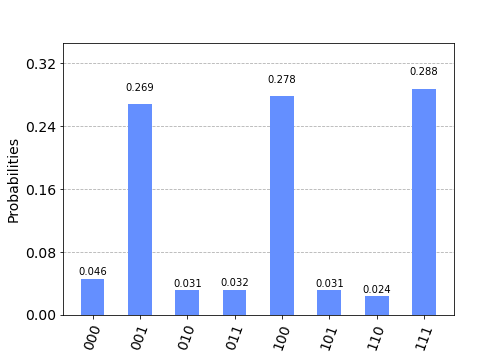
\includegraphics[scale = 0.75]{../Demonstration/img/simulated_3SAT.PNG}
	\caption{The simulated results plotted directely in a Jupyter notebook.}
\end{figure}

Now we will send off this circuit to an actual device. Make sure you pick an device from the IBMQ website that supports at the least 13 qubits.

\begin{verbatim}
from qiskit import IBMQ
IBMQ.load_account()
provider = IBMQ.get_provider(hub='ibm-q')
backend = provider.get_backend('ibmq_16_melbourne')
\end{verbatim}

Here we perform a manual transpile, which turns our algorithms in the needed gates to perform the Grover search algorithm for example. In this case, you are able to see the results of this transpile in text format under the code.

\begin{verbatim}
from qiskit.compiler import transpile


grover_compiled =transpile(result['circuit'],backend=backend, 
optimization_level=3)

print('gates = ', grover_compiled.count_ops())
print('depth = ', grover_compiled.depth())
\end{verbatim}

\begin{verbatim}
gates =  OrderedDict([('cx', 397), ('u2', 176), ('u1', 68), ('u3', 48),
('measure', 3), ('barrier', 2)])
depth =  431
\end{verbatim}

Once the circuit has run successfully you are able to view the result on the website of ibmqexperience in nicely put together format as visible from figure.

\begin{verbatim}
job = execute(result['circuit'], backend = backend , shots = 1024)
from qiskit.tools.monitor import job_monitor
job_monitor(job)
\end{verbatim}

Hopefully you will install Qiskit yourself and try these experiments out free-of-charge.



\begin{figure}
	\centering
	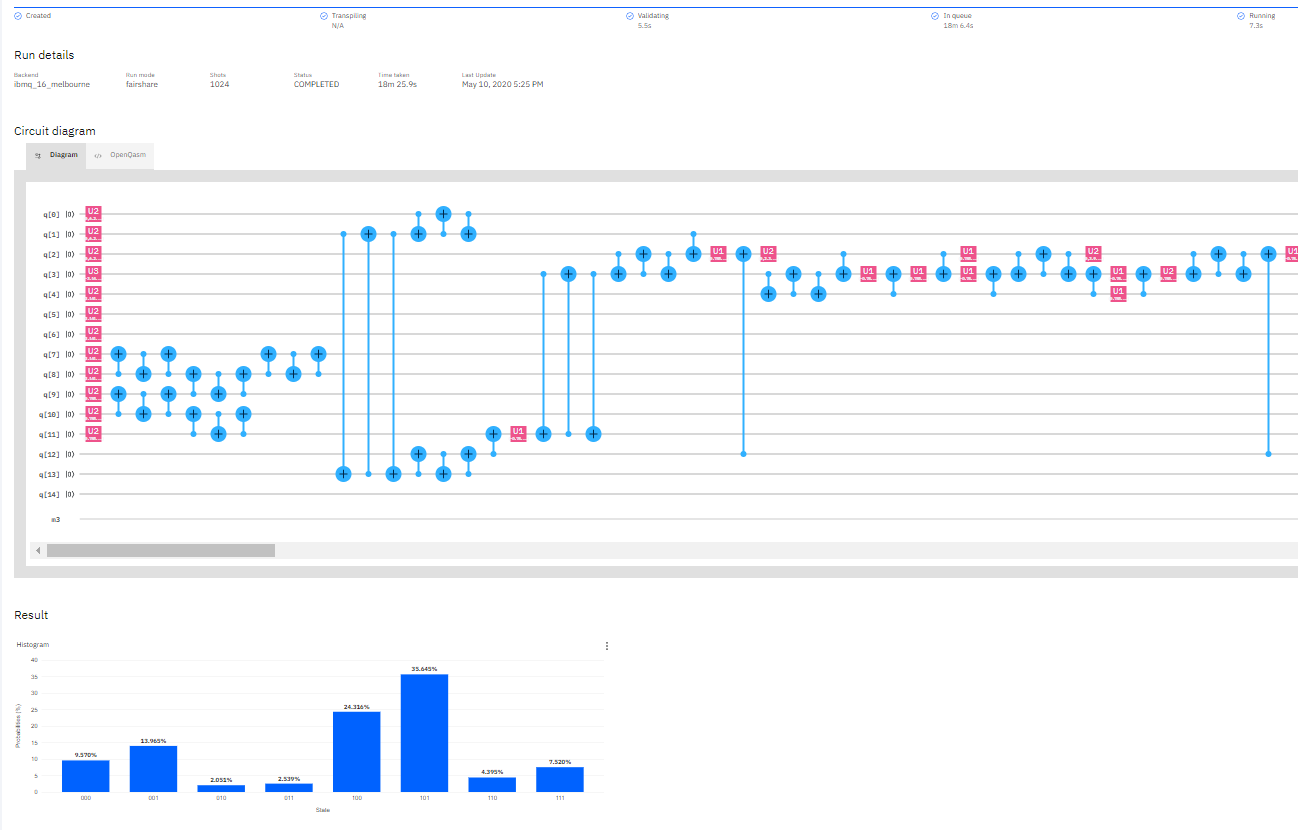
\includegraphics[scale = 0.50]{../Demonstration/img/ibmq_result.PNG}
	\caption{This is the visual result of running the practical version of this paper and displaying it on the ibmq website.}
\end{figure}
